\documentclass[10pt,letterpaper]{article}

\usepackage[utf8]{inputenc}
\usepackage[spanish,es-nodecimaldot]{babel}
\usepackage{amsmath}
\usepackage{amssymb}
\usepackage{graphicx}
\usepackage{mathtools}

\usepackage{multicol}

\usepackage{enumitem}

\usepackage[top=1in, bottom=1in, left=1in, right=1in]{geometry}

\renewcommand{\arraystretch}{1.5}

\begin{document}

\begin{titlepage}
    \centering

    {\scshape\LARGE Universidad Nacional Autónoma de México \par}

    \vspace{1cm}
    {\scshape\Large Facultad de Ciencias\par}
    \vspace{1.5cm}

    \begin{center}
        
\includegraphics[scale=.1]{../../assets/img/logo.png}
    \end{center}

    \vspace{.8 cm}

    {\LARGE Tarea 06: \par}
    {\huge\bfseries Estrategias evolutivas\par}

    \vspace{0.5cm}
    \large{\itshape{Pablo A. Trinidad Paz}} \small{ - 419004279}

    \vfill

    Trabajo presentado como parte del curso de
    \textbf{Cómputo Evolutivo}
    impartido por el profesor \textbf{Mario Iván Jaen Márquez}. \par
    \vspace{0.5cm}
    Fecha de entrega: \textbf{Jueves 4 de Abril de 2019}.
\end{titlepage}

\begin{enumerate}
    \item \textbf{[Ejercicio de programación]} Escribe una función que genere números
          pseudo-aleatorios de las distribución normal estándar $N(0, 1)$ a partir de
          números uniformemente distribuidos. Indica el método usado. \\[\baselineskip]

        \textbf{Solución:} Se implementó el método de muestreo de números pseudo-aleatorios
        descrito por Box-Muller\footnote{https://en.wikipedia.org/wiki/Box-Muller\_transform}.
        A continuación se presentan los resultados de la implementación comparados con el
        método $\mathrm{random.gauss(0, 1)}$ de la librería estándar de Python.
        \begin{center}
            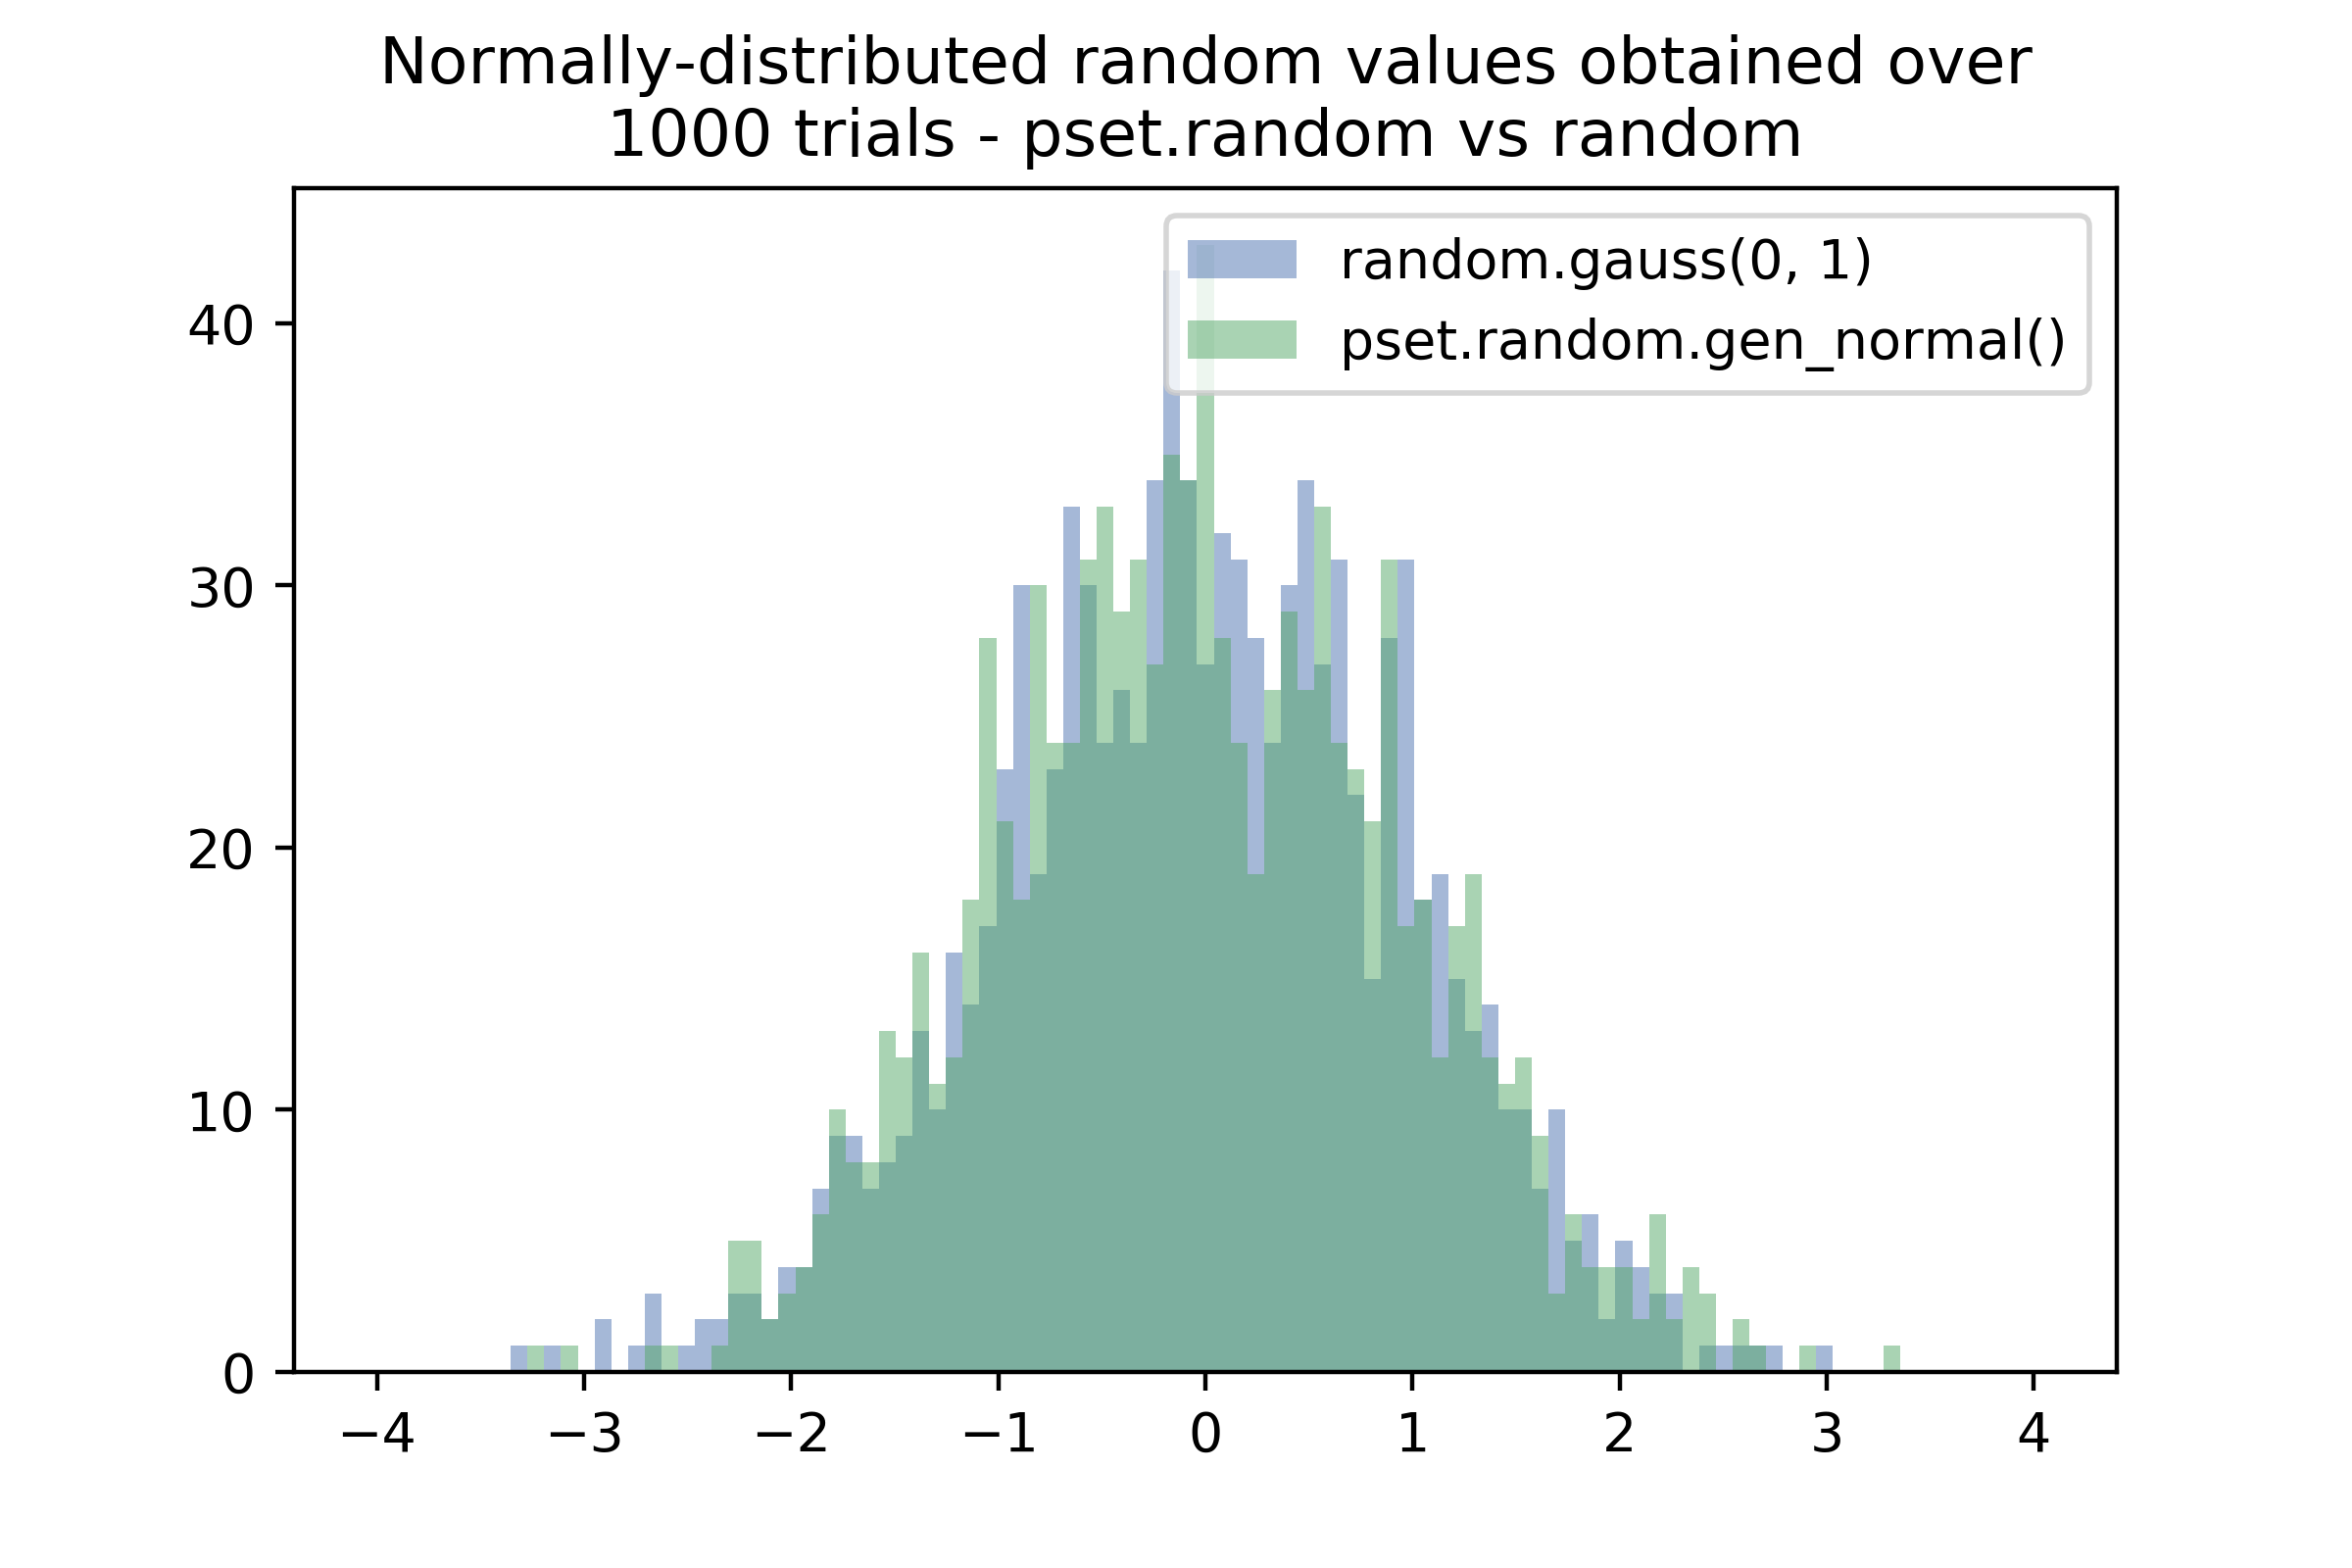
\includegraphics[scale=.6]{./assets/ex1-results1.png}
        \end{center}
        \begin{center}
            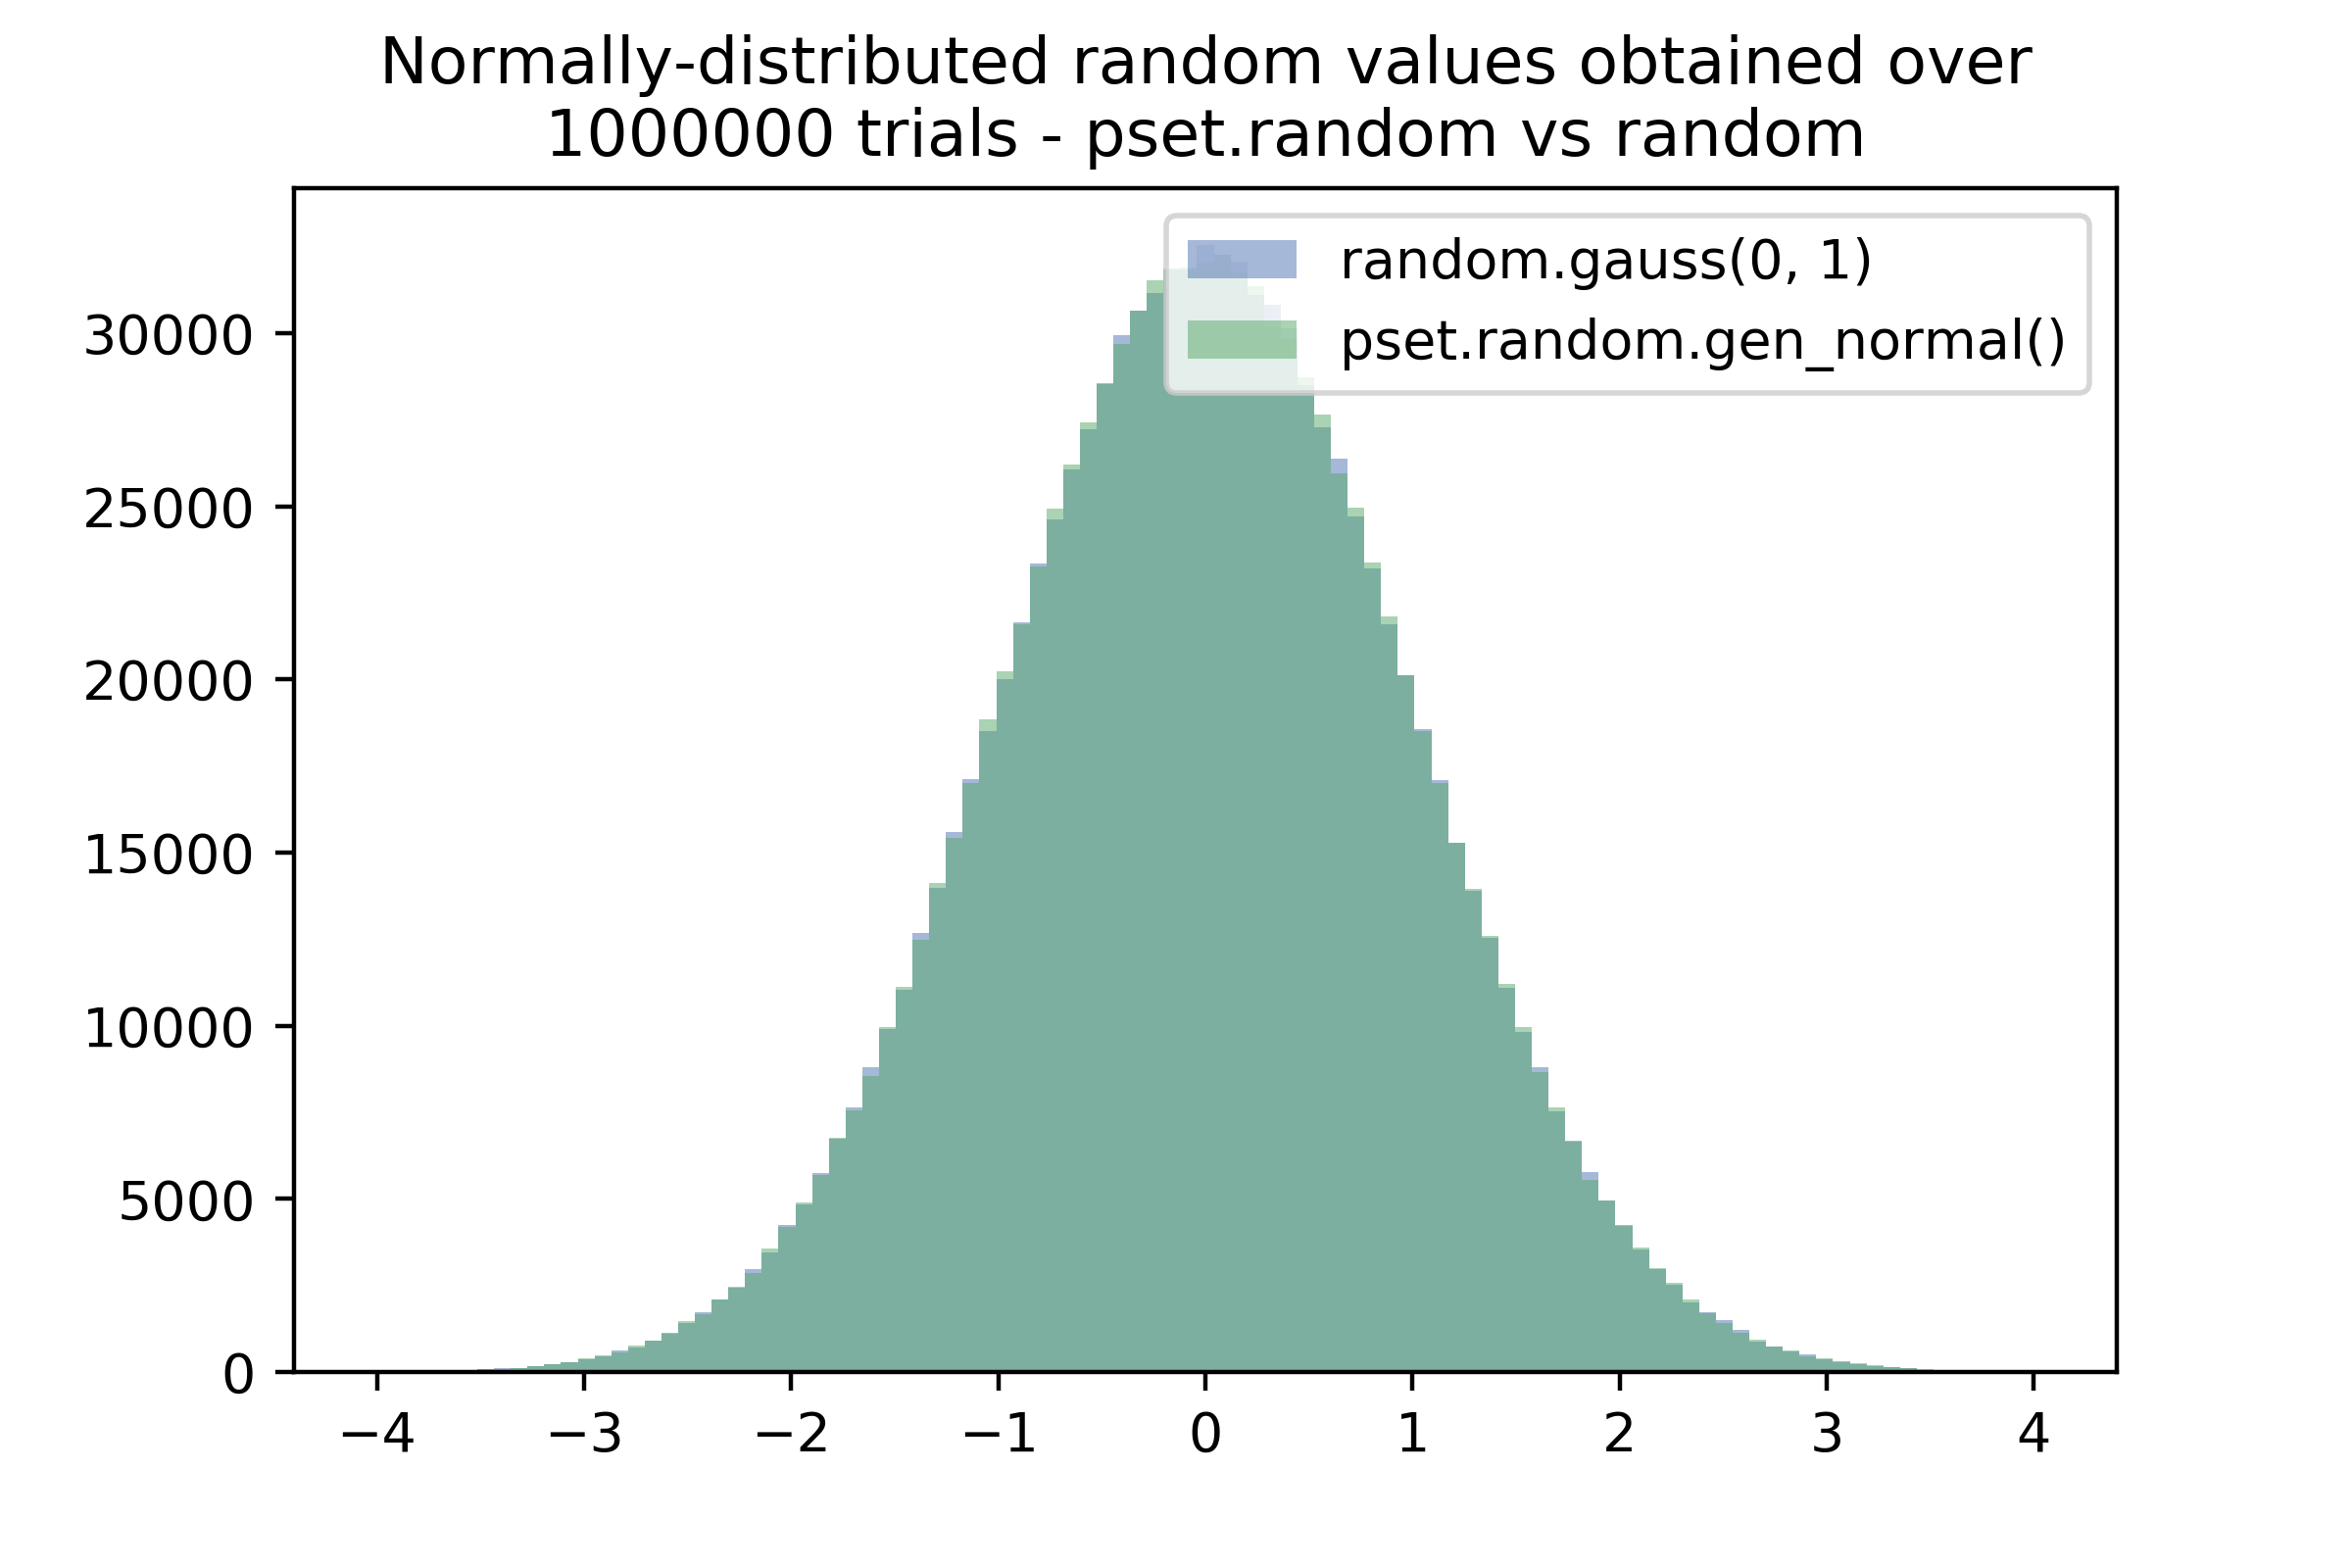
\includegraphics[scale=.6]{./assets/ex1-results2.png}
        \end{center}

    \clearpage
    \item \textbf{[Ejercicio de programación]} Implementa el algoritmo (1+1)-ES. Prueba
          tu algoritmo sobre la función \textit{Sphere}, la cuál es una función unimodal
          $d$-dimensional definida como:

        \begin{equation*} \begin{split} \begin{gathered}
            f(\vec{x}) = \sum_{i=1}^d x_i^2
        \end{gathered} \end{split} \end{equation*}

        Donde cada $x_i \in [-100, 100]$. Utiliza un parámetro $\sigma = 1$ y un punto
        inicial $\vec{x} = (x_1, ..., x_d) = (-99,...,-99)$

        \begin{enumerate}
            \item Ejecuta tu algoritmo para $d=10$ y para $d=100$. ¿Qué tan cerca del óptimo
            converge y qué tan rápido?

            \textbf{Respuesta:} Para $d=10$ con una precisión de $0.01$ y un máximo de $10^6$ iteraciones,
            el algoritmo concluye después $413$ mutaciones exitosas debido a haber alcanzado el número
            máximo de iteraciones con un valor promedio para cada $x_i$ de $-0.068264$
            y un fitness de $0.34359$ (el cual no cumple con la precisión).
            Para $d=100$ con la misma precisión, el algoritmo concluye después de $1296$
            mutaciones exitosas con un valor promedio para cada $x_i$ de $0.03281650$ y fitness de
            $125.16605$ (nuevamente lejano al óptimo y terminando debido al número máximo de iteraciones).

            \item Implementa la regla del $1/5$ y vuelve a ejecutar tu algoritmo. ¿Qué diferencias
            observas respecto a la ejecución anterior?

            \textbf{Respuesta:} La diferencia es fundamental en el sentido de que los algoritmos sí
            convergieron y en menos iteraciones que el límite permitía ($10^6$). Aproximadamente
            el $\sim 20\%$ de las mutaciones fueron exitosas en ambos casos a comparación del caso
            anterior donde menos del $0.001\%$ de las mutaciones fueron exitosas. En ambos casos se
            logró obtener fitness bajo la precisión solicitada: para $d=10$ se obtuvo $0.00907$ y para
            $d=100$ se obtuvo $0.00987$ con $515$ y $22,867$ iteraciones respectivamente y $120$ y $5,715$
            mutaciones exitosas respectivamente.
        \end{enumerate}

        \begin{center}
            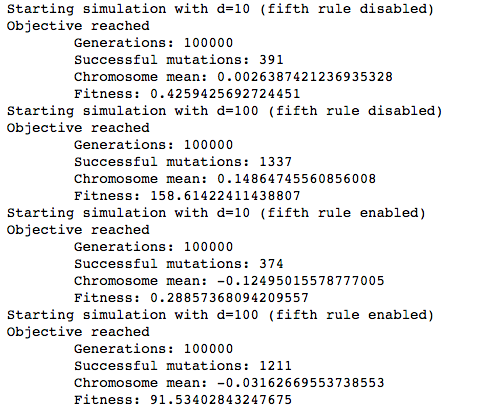
\includegraphics[scale=.6]{./assets/ex-2.png}
        \end{center}

    \clearpage
    \item \textbf{[Ejercicio de programación]} Implementa el algoritmo $(\mu + \lambda)$-ES
          usando mutación no correlacionada (una sola $\sigma$ para todas las dimensiones
          del problema). Para adaptar el tamaño de la mutación de $\sigma$ usa la recomendación
          dada en clases $\tau = 1/\sqrt{d}$. Prueba tu algoritmo en la función \textit{Sphere}
          y también en la función \textit{Ackley}, definida como:

          \begin{equation*} \begin{split} \begin{gathered}
              f(\vec{x}) = -20 \cdot \exp
                \Bigg(-0.2 \cdot \sqrt{\frac{1}{d} \cdot \sum_{i=1}^d x_i^2} \Bigg) -
                \exp \Bigg(\frac{1}{d} \cdot \sum_{i=1}^d \cos{(2 \pi x_i)}\Bigg) +
                20 + \exp (1)
          \end{gathered} \end{split} \end{equation*}

          donde cada $x_i \in [-30, 30]$. Prueba con diferntes valores de $\mu$ y -$\lambda$
          hasta alcanzar convergencia al óptimo global con un error por debajo de $0.001$.
          Puedes usar la recomendación de parámetros $\frac{\lambda}{\mu} \approx 7$.

        \begin{enumerate}
            \item Ejecuta tu algoritmo en $d=2$ y grafica los contornos de nivel de
                la función en los nivelos de $f(x): 2, 4, 6, 8, 100, 12, 14, 16, 18$ y $20$.
                \begin{center}
                    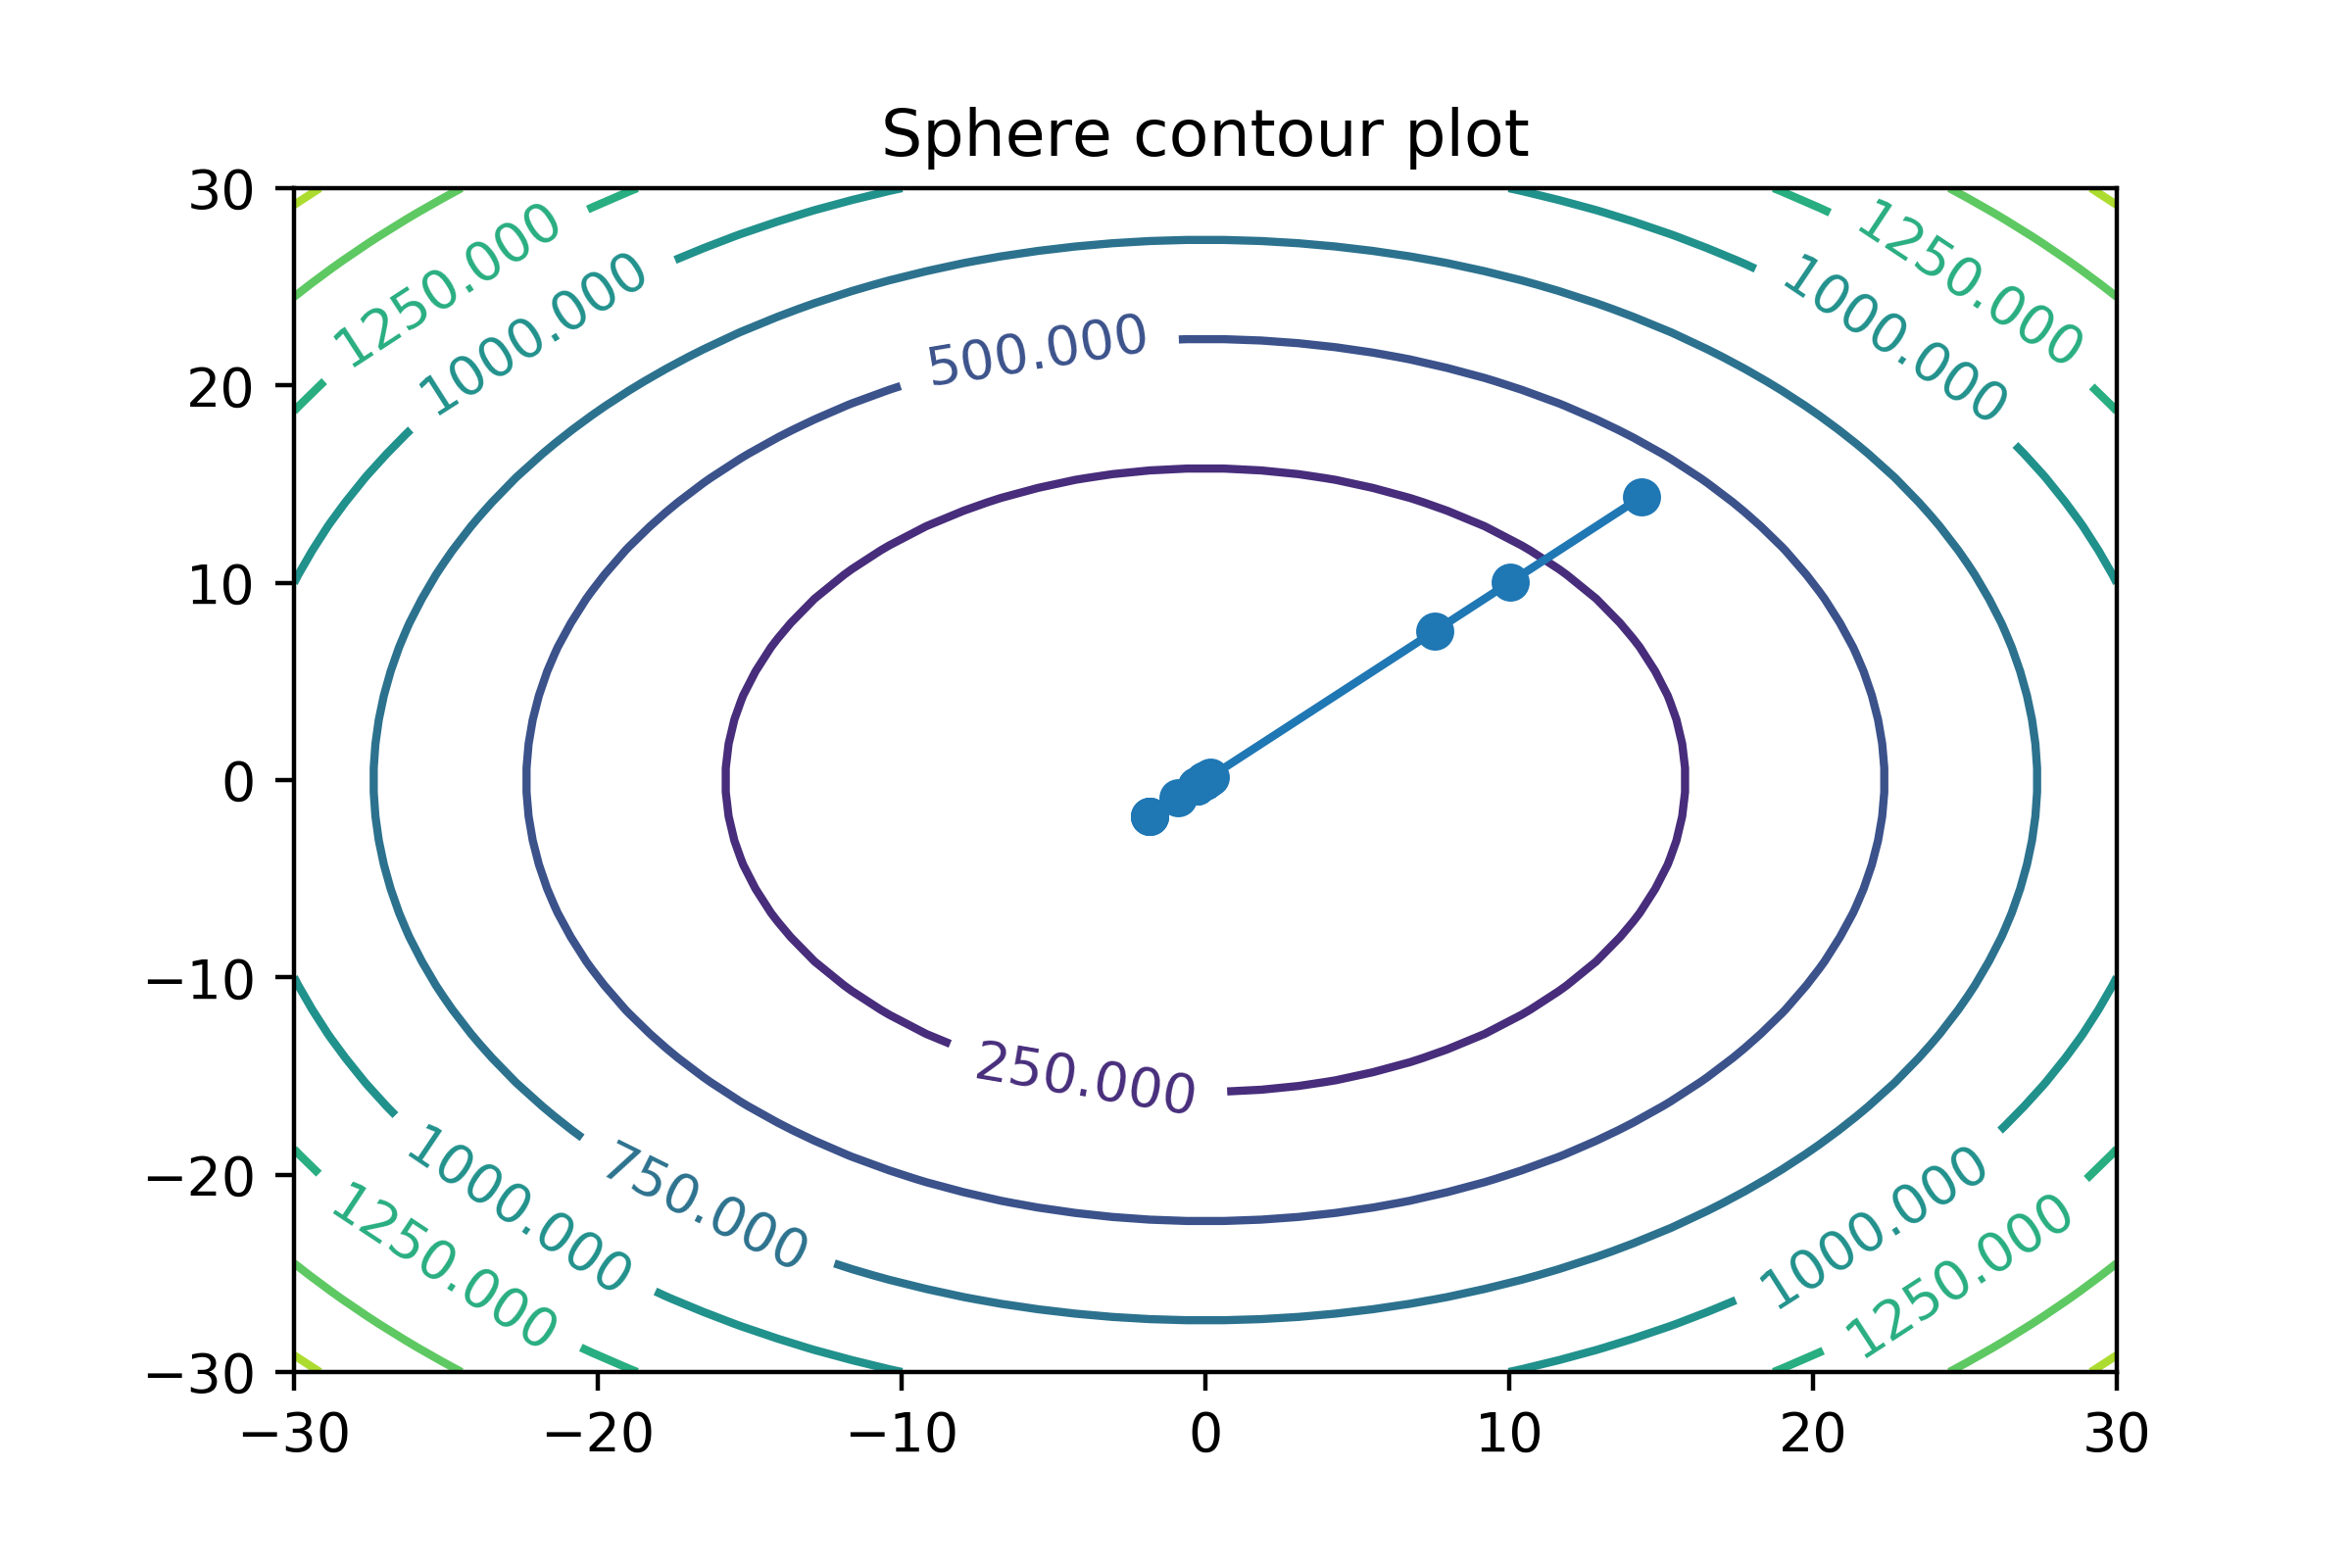
\includegraphics[scale=.6]{./assets/ex3-a-sphere.png}
                \end{center}
                \begin{center}
                    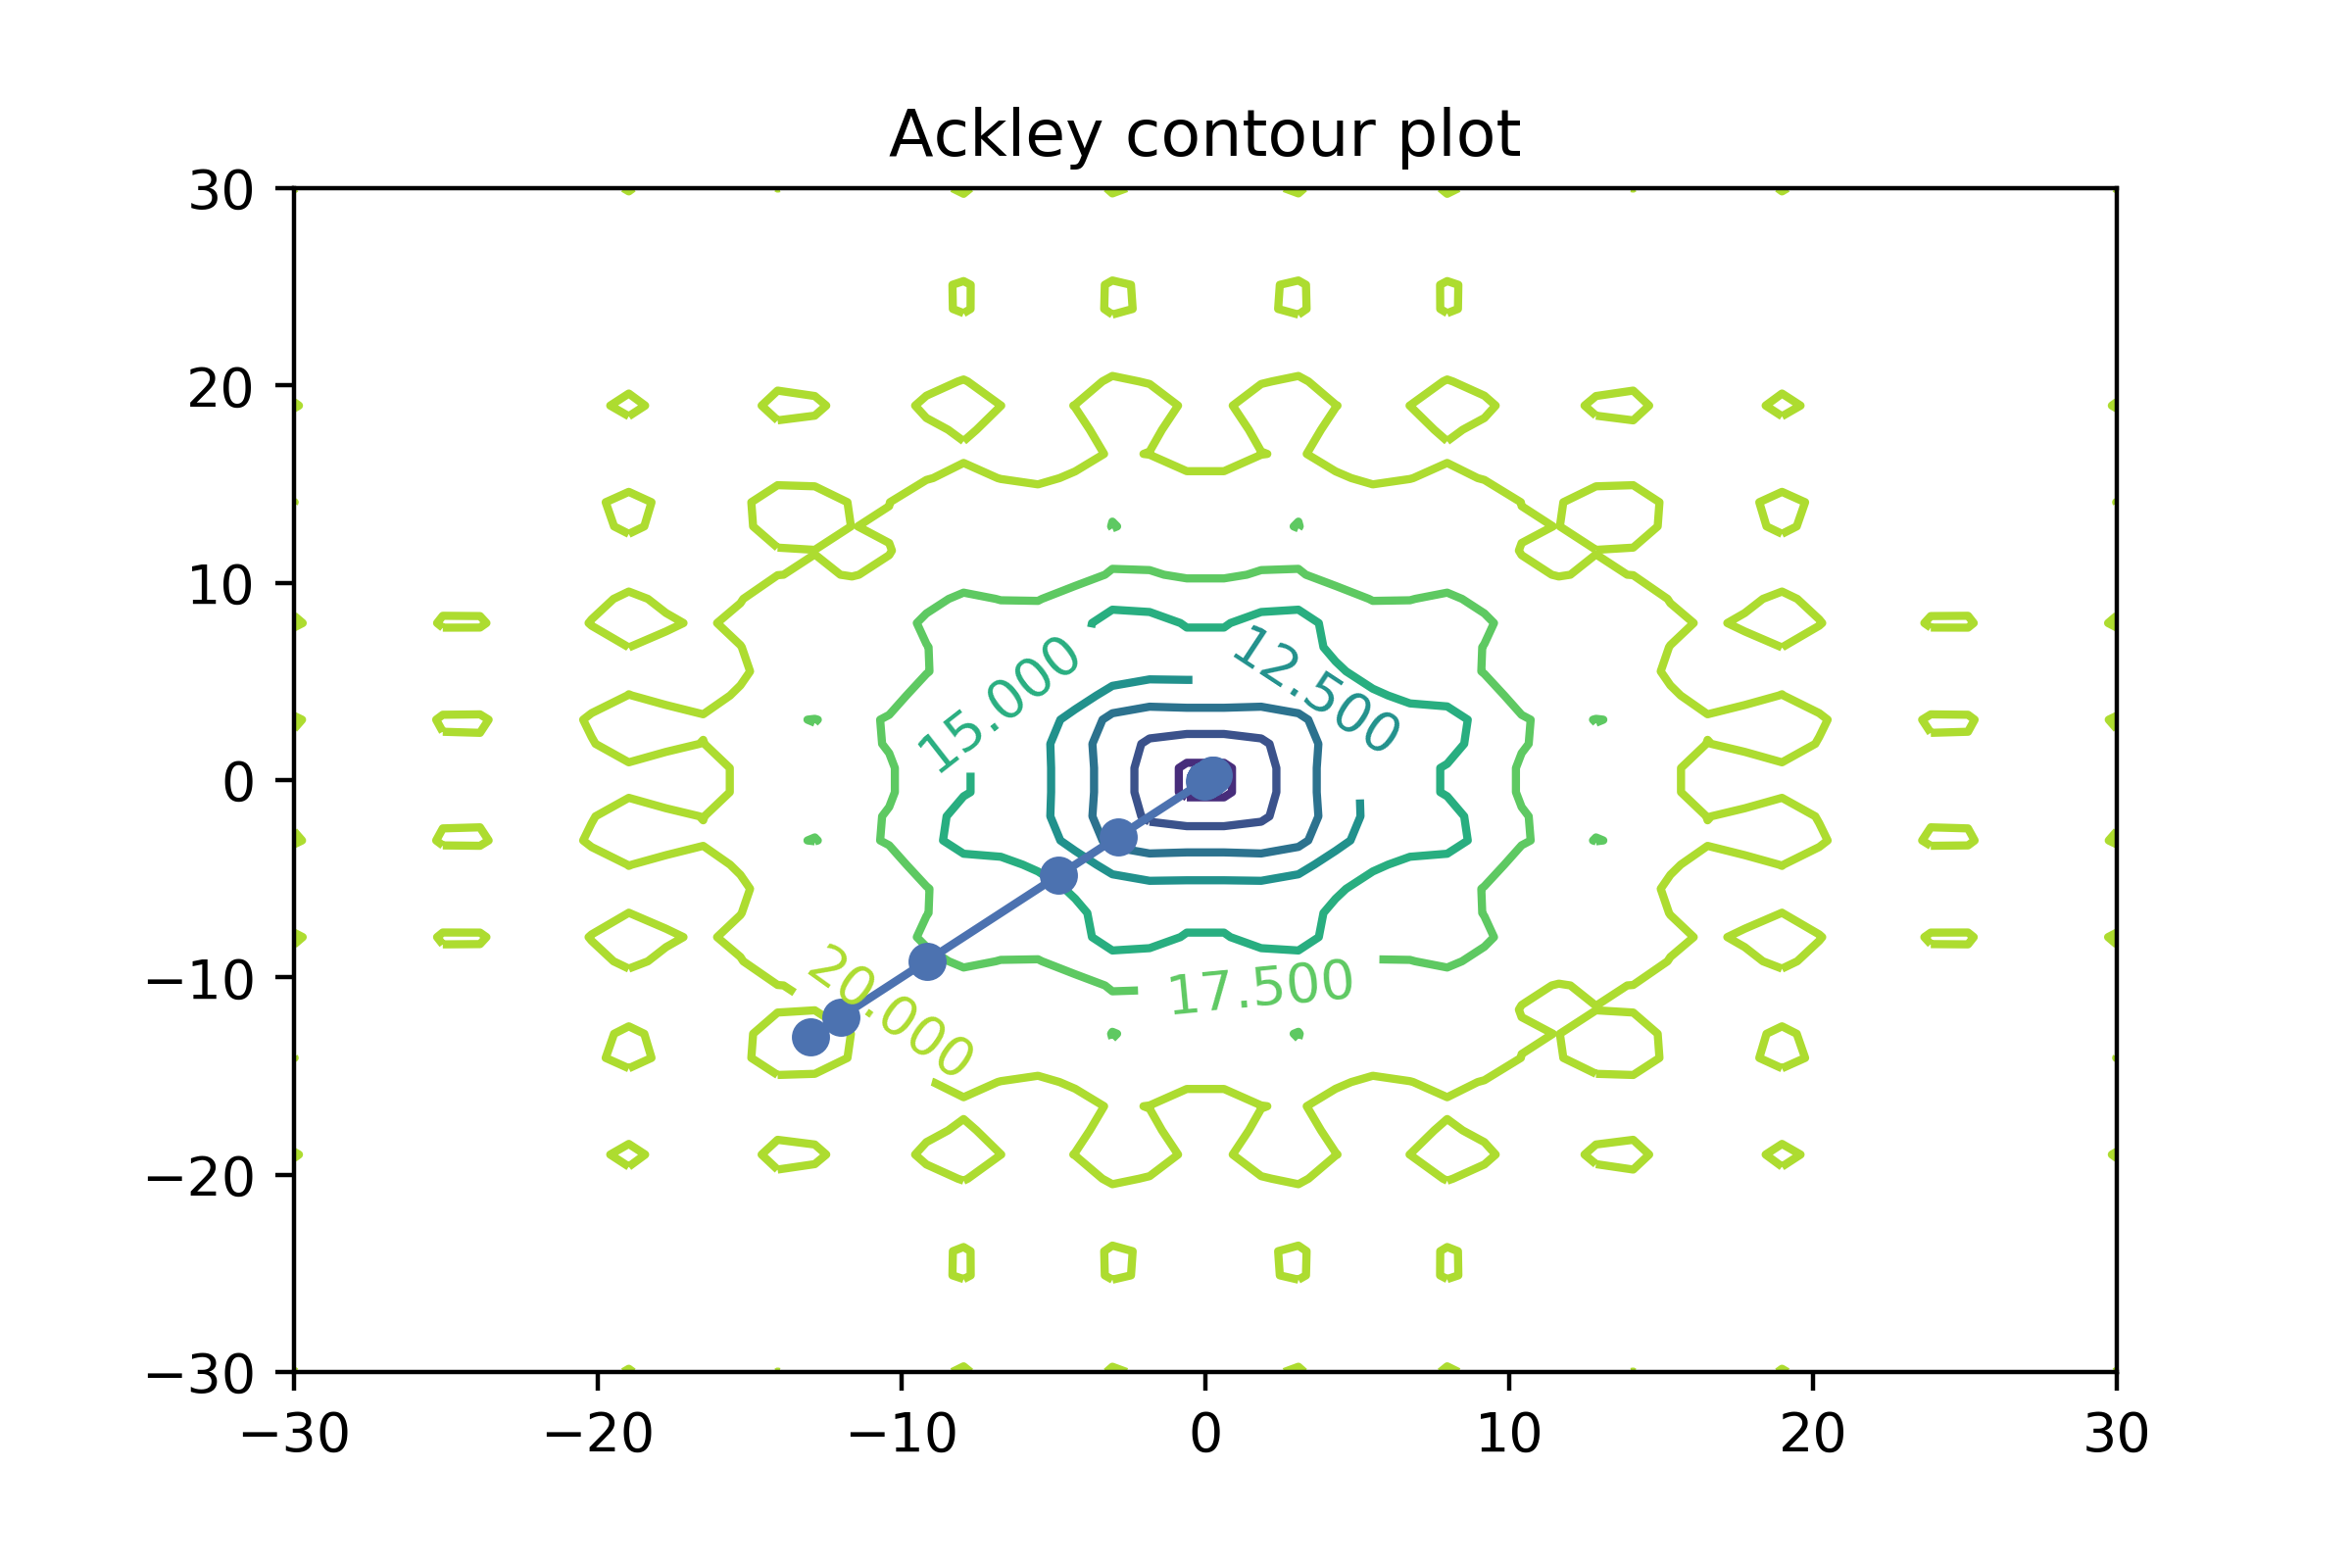
\includegraphics[scale=.6]{./assets/ex3-a-ackley.png}
                \end{center}
            \clearpage
            \item ¿Qué tan bien funciona $d=10$ respecto a la $(1+1)$-ES?

            \textbf{Respuesta:} Usando precisión de $0.001$ y $d=10$, $(\mu + \lambda)$-ES
            converge después de 74 generaciones mientras que $(1+1)$-ES lo hace después de
            667 generaciones con únicamente 146 mutaciones exitosas.

                \begin{center}
                    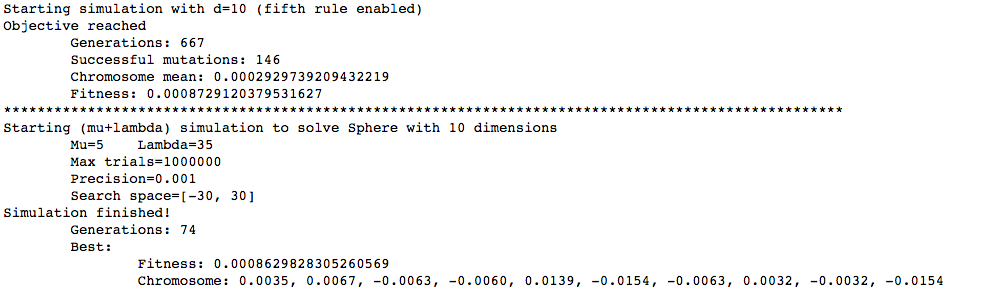
\includegraphics[scale=.5]{./assets/ex3-b.png}
                \end{center}
        \end{enumerate}
\end{enumerate}

\end{document}